\documentclass{article}
\usepackage{graphicx}
\usepackage{url}
\usepackage{natbib}
\usepackage{todonotes}
\title{A Topic Model of Climate Change Literature}
\title{Words, words, words: Mapping the Matter of Climate Change Literature}
\title{A Topography of Climate Change Research}
\author{Max Callaghan}
\begin{document}
\maketitle
\textbf{
To contribute to evidence-based policies on tackling climate change, the IPCC aims to comprehensively assess the relevant scientific literature \citep{IPCC2013}. With the size of this literature currently at least [x] times larger than at the time of the IPCC's first assessment report \citep{Houghton1990ClimateAssessment}, this task has become impossible without the aid of machine-reading. We collect over 300,000 abstracts from Web of Science (WoS) and Scopus, and develop a topic model in order to give an overview of this unmanageably large corpus. We find that new topics, such as [biochar] can be identified as they emerge, an application with a high potential for increasing the relevance and comprehensiveness of further IPCC reports.
}

The size of the scientific literature on climate change has expanded rapidly over the lifetime of the IPCC. While the first assessment report had around 7,000 articles to assess, 5,000 new articles are now published every month, bringing the total size of the literature to well over half a million papers, (Figure \ref{growth}). The increase in volume, velocity, and variety of content to be assessed has turned the task of the IPCC into a `Big Literature` challenge. To ask questions about the literature \textit{at scale}, we now need to employ computational techniques involving natural language processing.

Topic models are one such technique. A topic model learns the latent topics that structure a large corpus of documents, by leveraging the systematic co-occurrence of words across documents. Topics are distributions of words, and the topic mixture of each document explains the words observed in that document. This means that topic models can aid the understanding of large corpuses, and of the place of individual documents within them, by showing a document or corpus as a combination of 100 or so intelligible topics, rather than combinations of thousands of words.

The topic model presented here is a rough map of climate change research since 1985. It shows a broad outline of the topics that make up this research and how they relate to each other, and demonstrates how this has changed over time. This relief map does not replace the maps drawn by assessment-makers-as-cartographers for policymakers described in \citet{Edenhofer2015}. Rather, it supplements it by reducing the exploration time necessary and acting as a reference, to compare how the assessment reflects the literature. [Rather, it provides a vital anchor.]

While topic modelling has been employed to answer specific questions about small aspects of climate literature, e.g. \citep[e.g.][]{minx2016negative,Grubert2016}, this is the first application of topic models to gain an overview of the entire field.



\begin{figure}
	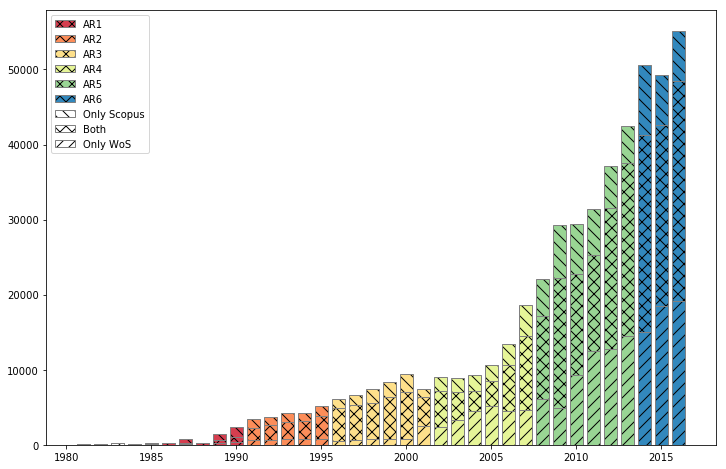
\includegraphics[width=\linewidth]{plots/wos_scopus_docs_time}
    \caption{Growth in relevant literature in WoS and Scopus}
    \label{growth}
\end{figure}




\section{Introduction}
\begin{itemize}
	\item Literature exploding, IPCC not keeping up \citep{minx2016learning}
    \item No systematic way of selecting references, no comprehensive assessment
    \item First step towards this is a map provided by topic models. 
    \item A map shows the places which the assessment makers need to navigate, leaving them to decide course. Computer assisted not computer decided.
    \item What is the topic structure of climate change research? How has it changed over time?
\end{itemize}

\section{Methodology}

\begin{itemize}
\item Model selection: NMF \citep{Lee1999}
\item How does it work? Advantages: Simple, scalable: better results than with other solutions, if only because it was possible to iterate with large document collections. LDA can be better but relies on tuning hyperparameters, hard to do with such big corpus
\item Topic model browser \citet{Chaney2012}
\item Human Validation: 
\item Compare topic space to keyword space. Reduces dimensionality, overcomes non-standardisation
\item Which topics get the most citations?

\end{itemize}

\section{Data}
\begin{itemize}
	\item Queries: use \citet{Grieneisen2011}, or take the best bits of \citet{Grieneisen2011} and \citet{Haunschild2016}?
    \item Sources: WoS, Scopus or both?
    \item Preprocessing: Remove punctuation, numbers, common, uncommon words, stemming
\end{itemize}

\section{Results}
\begin{itemize}
	\item The biggest topics are x and y
	\item These topics have grown, these have decreased
    \item X keywords fit into Y topics like so...
    \item Finding similar documents works across topics, rather than just by keywords, so better.
    \item Similar documents more or less likely to be across disciplinary boundaries ??
    \item Model selection validated by these measurements.
\end{itemize}

\section{Conclusion}
\begin{itemize}
	\item A very simple topic model provides an overview of the whole landscape.
    \item This allows researchers / assessment makers to identify areas that have grown recently
    \item Topic models aid document discovery, have the potential to contribute to more comprehensive assessments.
    \item Next steps for research: using topic models to assess the assessment process: find gaps etc.
\end{itemize}

\begin{figure}
	%\includegraphics{}
    \caption{Topic structure of climate change literature [network plot]}
\end{figure}

\begin{figure}
	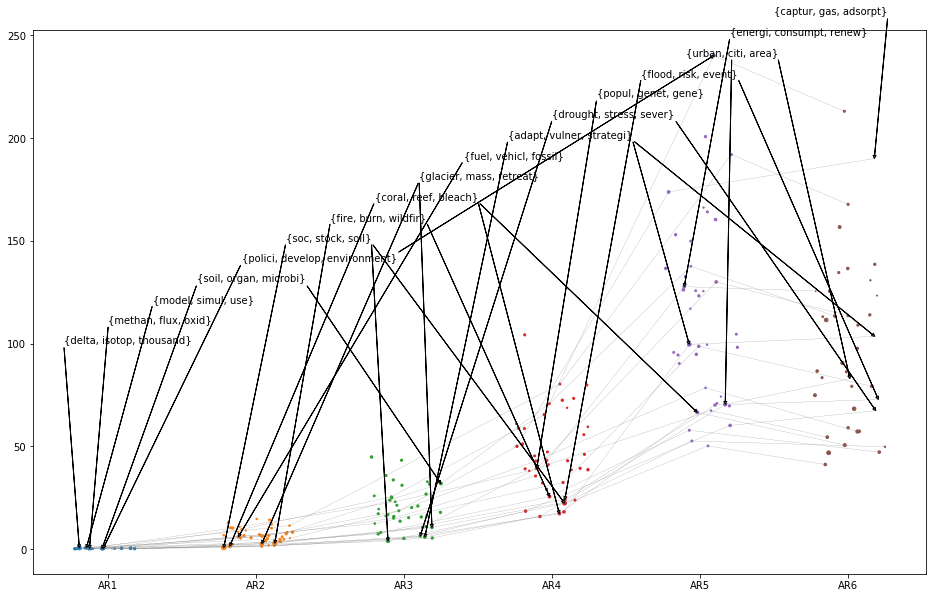
\includegraphics[width=\linewidth]{plots/hot_topics}
    \caption{Topic growth over time. The 3 topics in each assessment period that grew by the largest amount are labelled}
\end{figure}

\begin{figure}
	%\includegraphics{}
    \caption{Focus on [biochar?] showing document with highlighted words}
\end{figure}

\begin{figure}
	%\includegraphics{}
    \caption{Model validation graph, showing error for different topic numbers, feature numbers}
\end{figure}


\begin{figure}
	%\includegraphics{}
    \caption{Some relation of topics to other features of dataset: e.g. most interdisciplinary journals and least, or so...}
\end{figure}



\listoffigures

\bibliography{Mendeley.bib}
\bibliographystyle{apalike}

\end{document}

